\documentclass[conference,onecolumn,12pt]{IEEEtran}
\IEEEoverridecommandlockouts
\hyphenation{op-tical net-works semi-conduc-tor}
\usepackage{cite}
\usepackage{fancyhdr}
\usepackage{lipsum}
\usepackage{amsmath,amssymb,amsfonts}
\usepackage{algorithmic}
\usepackage{graphicx}
\usepackage{textcomp}
\usepackage{comment}
\usepackage{xcolor}
\usepackage{float}
\usepackage{svg}
\usepackage{tabularx}
\usepackage{hyperref}
\usepackage{breqn}
\usepackage{siunitx}
\usepackage[natbib=true,style=trad-unsrt,backend=biber]{biblatex}
\usepackage{minted}
\renewcommand{\baselinestretch}{1.5}
\usepackage{caption}


\setminted{
    baselinestretch=1.0, % Controls the line spacing inside minted blocks
    fontsize=\small, % Sets the font size
    frame=single, % Adds a frame around the code
    framesep=10pt % Controls the space between code and frame
}

\usepackage{circuitikz}

\addbibresource{references.bib}

\renewcommand{\tablename}{Tabla} 
\renewcommand{\abstractname}{\large Resumen}
\renewcommand{\IEEEkeywordsname}{\large Palabras Clave}
\renewcommand{\figurename}{Fig.}
\numberwithin{equation}{subsection}

\usepackage{titlesec}

% Change section title size
\titleformat{\section}
  {\centering \large} % Change this to \Large, \huge, etc.
  {\thesection}{1em}{}  

% Change subsection title size
\titleformat{\subsection}
  {\centering \large}
  {\thesubsection}{1em}{}

% Change subsubsection title size
\titleformat{\subsubsection}
  {\centering \large}
  {\thesubsubsection}{1em}{}



%-------------------------No tocar de aqui para atras-----------

%-------------------------Título y nombres-----------
\begin{document}


\title{Proyecto 2: Control de péndulo amortiguado a hélice}

\author{
\IEEEauthorblockN{
\fontsize{12pt}{12pt}\selectfont Wilberth Daniel Gutiérrez Montero \IEEEauthorrefmark{1}, Ronald Esteban Duarte Barrantes \IEEEauthorrefmark{2} \\
Nagel Eduardo Mejía Segura\IEEEauthorrefmark{3}
}
\IEEEauthorblockA{
\fontsize{12pt}{12pt}\selectfont Escuela de Ingeniería en Electrónica, Instituto Tecnológico de Costa Rica. \\
\fontsize{12pt}{12pt}\selectfont Emails: wil.gutierrez@estudiantec.cr \IEEEauthorrefmark{1},\\ ronald@estudiantec.cr \IEEEauthorrefmark{2}, nagelmese@estudiantec.cr \IEEEauthorrefmark{3} 
}
}


\maketitle
\fontsize{12pt}{12pt}\selectfont
\thispagestyle{plain}
\pagestyle{plain}
%-------------------------Inicio-----------

\begin{abstract}
\fontsize{12pt}{12pt}\selectfont
En primeras instancias se trabaja con  sistema de segundo orden el cual es el mas cercano a la planta PAMH. El cual sera de utilidad para la identificación y diseño de los distintos controladores, encargados de generar una respuesta deseada en la planta, en los cuales se obtuvieron tiempos de estabilización de 5 segundos, y eliminación de perturbaciones. Todos los controladores fueron implementados en el sistema físico utilizando la herramienta de PASCAL. Se evaluaron principalmente en función del tiempo de respuesta, estabilidad y capacidad para eliminar perturbaciones, obteniendo resultados favorables para el método con realimentación de estados con LQR.

\end{abstract}

%-------------------------Palabras clave-----------
\begin{IEEEkeywords}
\fontsize{12pt}{12pt}\selectfont
 cancelación de polos, I-PD, integrador, REI, PAHM, PID.

\end{IEEEkeywords}

\section{Introducción}
\fontsize{12pt}{12pt}\selectfont
\IEEEPARstart{E}l Péndulo Amortiguado a Hélice (PAMH) es una planta que consta de un péndulo con una hélice en uno de sus extremos, y una masa pequeño en el otro extremo, la cual (sin control) genera un movimiento oscilatorio. En este informe se presentan tres tipos de controles distinto los cuales se encargan de estabilizar la hélice en un punto requerido, para ello se desarrollaron los controladores como el PID (Manual), PID (IMC), I-PD (LQR), I-PD (Ackerman), REI (LQR) y REI (Ackerman) esto mediante la utilización de las herramientas Ident, Sisotool y Simulink de MATLAB. Estas herramientas permiten la identificación del sistema, el diseño del controlador mediante la modificación del lugar de las raíces y la implementación del sistema controlado en un diagrama de bloques.
\newpage
\section{Identificación y resultados}

\subsection{Identificación del Sistema}

Primero, por medio del programa PASCAL, se generaron los datos para la identificación del sistema, se introdujo al sistema una entrada constante por 40 segundos para permitir la estabilización del sistema, a partir de ese momento se afectó al sistema con una perturbación por unos 20 segundos, la entrada vuelve a 0 terminando con las mediciones. En la Fig. \ref{fig:pamhident} se observa la respuesta del sistema.

\begin{figure}[htbp]
    \centering
    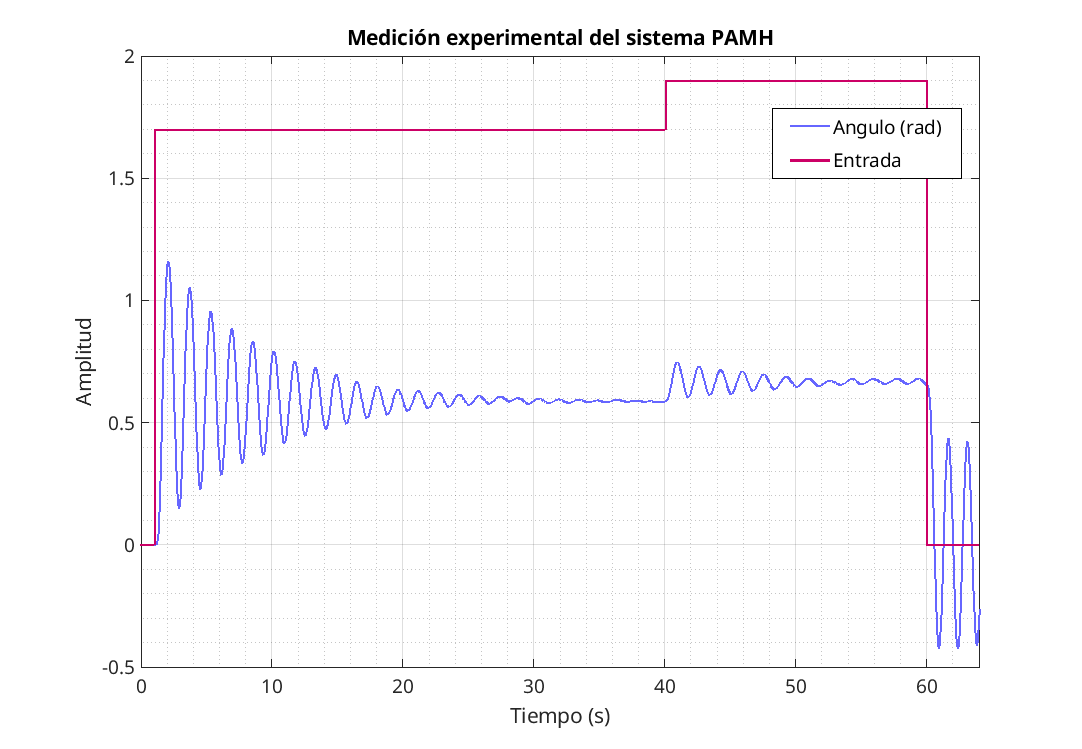
\includegraphics[width=1\linewidth]{fig/pamhident.png}
    \caption{Mediciones del sistema PAMH}
    \label{fig:pamhident}
\end{figure}

Cabe resaltar que el sistema presenta un pequeño retardo de unos 220 ms. Para la identificación del sistema se utilizó el System Identification de MATLAB, donde se utilizó un rango de 36 a 38 segundos, momentos donde se estabiliza el sistema. Para asegurar el mayor porcentaje de coincidencia con el sistema fisico, se utilizó el delay, sin embargo, para el modelo no se tomó en cuenta, obteniendo el modelo de la Ec. \ref{ec:modelpamh}

\begin{equation}
    P(s) = \frac{5.3881}{s^2 + 0.2673s + 15.33}
    \label{ec:modelpamh}
\end{equation}

En la Fig. \ref{fig:pamhmodel} se denota el comportamiento del modelo, ante la misma entrada efectuada en el sistema fisico. Si bien, no es un modelo exacto, se logra obtener el mismo comportamiento oscilatorio (frecuencia natural) con su respectiva atenuación.

\begin{figure}[htbp]
    \centering
    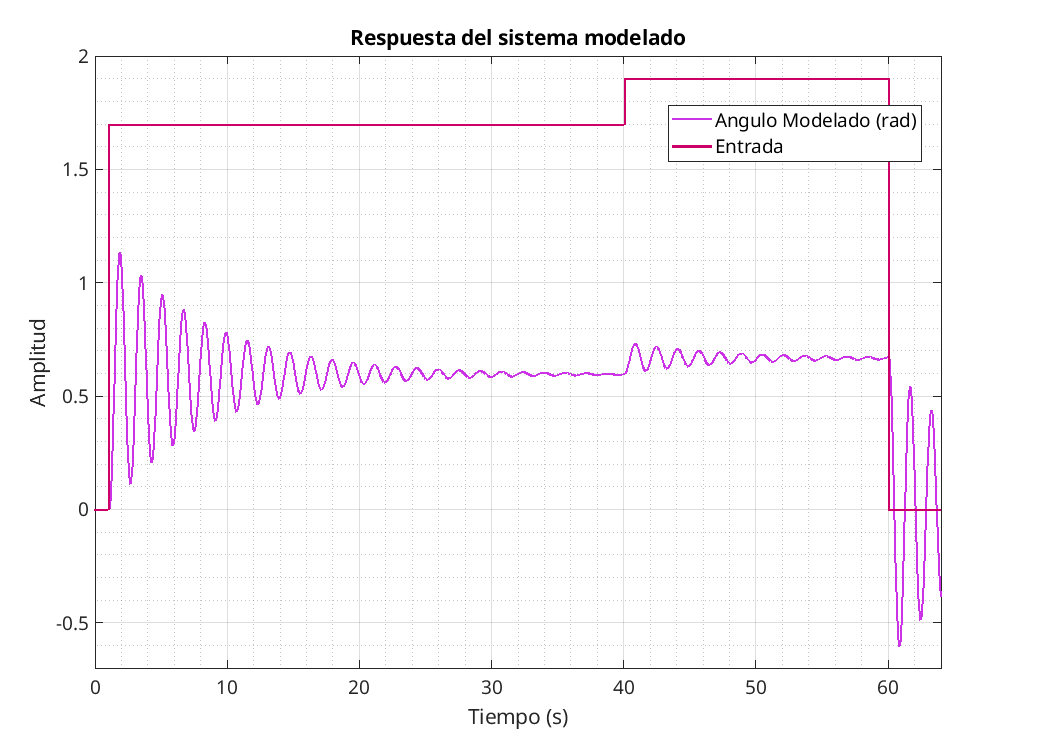
\includegraphics[width=1\linewidth]{fig/pamhmodel.png}
    \caption{Mediciones del sistema PAMH}
    \label{fig:pamhmodel}
\end{figure}

\subsection{Diseño de Controlador PID}

\subsubsection{Método manual}

Para el diseño del controlador por el método manual, se agrega un integrador, un polo real y un par de ceros complejos para la cancelación de polos. Los ceros complejos se ubican en las raíces del modelo, tal que usando la herramienta "eig()" de matlab e introduciendo el modelo previamente obtenido, se obtienen las raíces de la Ec. \ref{eq:polosPID}.

\begin{equation}
    z_{1,2} = -0.1336 \pm 0.3.9127j \ \ \ \ 
    \label{eq:polosPID}
\end{equation}

Posteriormente, se modificó la ganancia para cumplir con los requerimientos de diseño tal que el controlador final se observa en la Ec. \ref{eq:cPID} y el lugar de las raíces en la Fig. \ref{fig:pamhsys_pidroot}.

\begin{figure}[htbp]
    \centering
    \includegraphics[width=0.9\linewidth]{fig/PIDMAN_TUNE.png}
    \caption{Lugar de las raíces del sistema con controlador PID manual}
    \label{fig:pamhsys_pidroot}
\end{figure}

\begin{equation}
    C_{PIDmanual} = \frac{0.159(s^2+0.267s+15.3)}{s(s+1.6)} \ \ \ \ 
    \label{eq:cPID}
\end{equation}

Donde se obtiene un tiempo de estabilización de 4.67 segundos y un sobreimpulso de 0.45\%, tal como se observa en la Fig. \ref{fig:pamhsys_pistep}.

\begin{figure}[!ht]
    \centering
    \includegraphics[width=0.9\linewidth]{fig/PIDMAN_STEPRES.png}
    \caption{Respuesta al impulso del sistema con controlador PID manual}
    \label{fig:pamhsys_pistep}
\end{figure}

Además por fracciones parciales se obtuvieron las constantes Kp, Ki, Kd y N, como se muestra en la Ec. \ref{eq:pids_ks}.

\begin{equation}
    K_p = -0.9240\ \ \ \ K_i = 1.5204 \ \ \ \ K_d = 0.6769\ \ \ \ N = 1.6
    \label{eq:pids_ks}
\end{equation}

\subsubsection{Método IMC}

El método IMC utiliza el internal model control tuning de matlab para generar un controlador automáticamente utilizando el orden de controlador deseado y la constante de tiempo dominante de lazo cerrado. Tal que el orden utilizado es de 2, y la constante de tiempo dominante de lazo cerrado se estableció en 0.82, de modo que, el controlador obtenido se observa en la Ec. \ref{eq:cPIDimc}

\begin{equation}
    C_{PIDIMC} = \frac{0.27602(s^2+0.267s+15.3)}{s(s+2.44)} \ \ \ \ 
    \label{eq:cPIDimc}
\end{equation}

Donde se obtiene un tiempo de estabilización de 4.78 segundos y un sobreimpulso nulo, tal como se observa en la Fig. \ref{fig:pidimcstep}.

\begin{figure}[!ht]
    \centering
    \includegraphics[width=0.9\linewidth]{fig/pidimc_step.png}
    \caption{Respuesta al impulso del sistema con controlador PID por IMC}
    \label{fig:pidimcstep}
\end{figure}

Además por fracciones parciales se obtuvieron las constantes Kp, Ki, Kd y N, como se muestra en la Ec. \ref{eq:pidimc_ks}.

\begin{equation}
    K_p = -0.6819\ \ \ \ K_i = 1.7371 \ \ \ \ K_d = 0.3928\ \ \ \ N = 2.439
    \label{eq:pidimc_ks}
\end{equation}

\subsection{Diseño de Controladores I-PD y REI}

Para ambos tipos de reguladores se utilizó el modelo de espacio de estados del sistema PAMH, en la Ec. \ref{eq:ss} se observa la forma canónica controlable del sistema.

\begin{equation}
    A = \begin{bmatrix}
0 & 1 \\
 -15.3273 &  -0.2673
\end{bmatrix} \ B=\begin{bmatrix}
 0 \\
 5.3881
\end{bmatrix} \ C = \begin{bmatrix}
1 & 0
\end{bmatrix}
\label{eq:ss}
\end{equation}

A partir de las matrices, se verificó que el sistema fuera controlable, por medio de la Ec. \ref{eq:ctrl}, donde se obtuvo un el rango de 3.

\begin{equation}
    rango \left( \begin{matrix}
        A & B \\
        -C & 0
    \end{matrix} \right) = 3
    \label{eq:ctrl}
\end{equation}

\subsubsection{Método Ackerman (Ubicación de polos)}

Para el método de ubicación se eligió un polo con su conjugado, los cuales se seleccionan cercano a los valores de polos que se deseo, para determinar el comportamiento del transitorio, además se seleccionó un polo alejado de los polos dominantes para generar el polinomio de tercer orden. Los polos seleccionados fueron los de la Ec. \ref{eq:polos}.

\begin{equation}
    p_{1,2} = -0.85 \pm 0.5j \ \ \ \ p_3 = -4
    \label{eq:polos}
\end{equation}

Por medio de MATLAB, se generaron las matrices y se utilizó el comando acker(), lo que generó la matriz de ganancia de control de la Ec. \ref{eq:k_acker} y la ganancia para la parte integral de la Ec. \ref{eq:ki_acker}.

\begin{equation}
   K = \begin{bmatrix}
       -1.4021 & 1.0083
   \end{bmatrix}
    \label{eq:k_acker}
\end{equation}

\begin{equation}
    K_i = 0.7220
    \label{eq:ki_acker}
\end{equation}

\subsubsection{Método LQR}

Para el diseño con el método LQR se generó la matriz $Q$ y $R$, esta ultima se seleccionó simplemente como 1, en cuanto a la $Q$ en la Ec. \ref{eq:q_lqr} se observan los valores seleccionados con el fin de ajustar los estados del sistema.

\begin{equation}
   Q = \begin{bmatrix}
       5 & 0 & 0 \\
       0 & 5 & 0 \\
       0 & 0 & 9.5 \\
   \end{bmatrix}
    \label{eq:q_lqr}
\end{equation}

Por medio del comando lqr() se generó la matriz de ganancia de control de la Ec. \ref{eq:k_lqr} y la ganancia para la parte integral de la Ec. \ref{eq:ki_lqr}.

\begin{equation}
   K = \begin{bmatrix}
       2.4546 & 2.3822
   \end{bmatrix}
    \label{eq:k_lqr}
\end{equation}

\begin{equation}
    K_i = 3.0822
    \label{eq:ki_lqr}
\end{equation}



\subsection{Comparación de Reguladores}

En la Tabla \ref{tab:comp_design} se observa una comparación de los distintos diseños, denotando los coeficientes así como los valores importantes en la estabilidad del sistema.

\begin{table}[htbp]
\centering
\caption{Comparacion de Reguladores Diseñados}
\label{tab:comp_design}
\begin{tabular}{|l|c|c|c|c|c|c|}
\hline
Caracteristica \textbackslash{}textbackslash Regulador & PID (Manual) & PID (IMC) & I-PD (LQR) & I-PD (Acker) & REI (LQR) & REI (Acker) \\ \hline
$K_p$                                                  &      -0.9240       & -0.6819          & 2.4546     & -1.4021      & 2.4546    & -1.4021     \\ \hline
$K_i$                                                  &    1.5204&  1.7371          & 3.0822     & 0.7220       & 3.0822    & 0.7220      \\ \hline
$K_d$                                                  &    0.6769          & 0.3928          & 2.3822     & 1.003        & 2.3822    & 1.0083      \\ \hline
$N$                                                    &     1.6         & 2.439          & 5          & 5            & NA        & NA          \\ \hline
Tiempo de Estabilización (s)                           & 4.67        &     4.78      & 4.861      & 4.661        & 4.881     & 4.861       \\ \hline
Porcentaje de Amortiguamiento (\%)                     & 0.45            &   0        & 0          & 1            & 0         & 0           \\ \hline
Elimina Perturbaciones                                 & Sí           & Sí        & Sí         & Sí           & Sí        & Sí          \\ \hline
\end{tabular}
\end{table}

\section{Implementación de Controladores}

Se implementaron los controladores por medio del programa PASCAL, para este caso se utilizaron los métodos que presentaron los tiempos más lentos, esto con el fin de no exigir demasiado al sistema, de este modo, se seleccionó el PID por IMC, I-PD por medio de ubicación de polos (Ackerman) y la REI por medio de LQR.



\subsection{Control por PID obtenido por IMC}

Para el controlador PID obtenido por IMC, se puede observar en la Fig .\ref{fig:pamhsys_pid} como el ángulo de salida presenta pequeñas oscilaciones que disminuyen con el tiempo, pese a esto, el controlador elimina satisfactoriamente las perturbaciones, presentando un leve impulso que rápidamente tiende al estado anterior.

\begin{figure}[htbp]
    \centering
    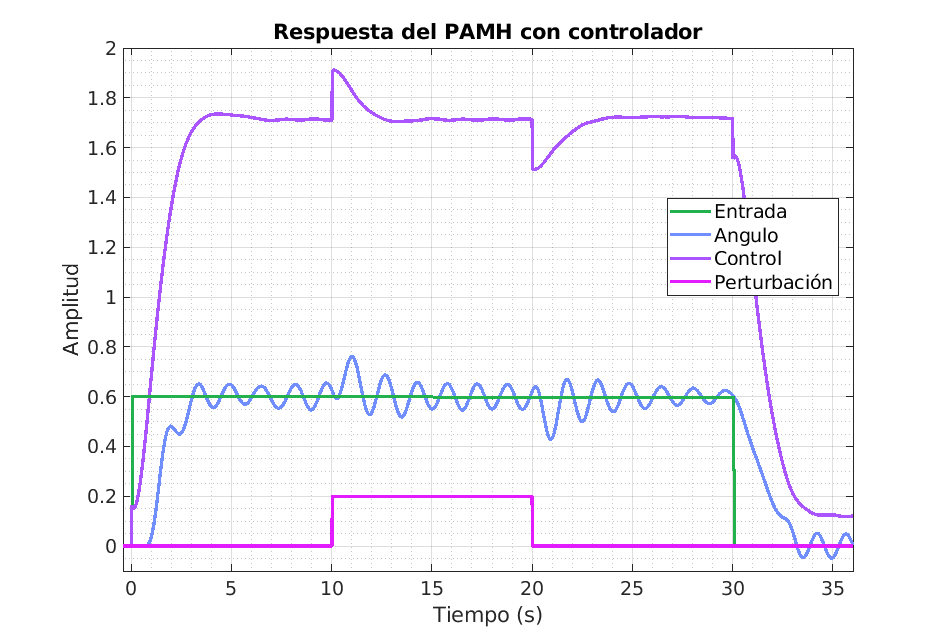
\includegraphics[width=1\linewidth]{fig/PAMH_PID2.png}
    \caption{Respuesta del sistema PAMH controlado con PID}
    \label{fig:pamhsys_pid}
\end{figure}

\subsection{Control por I-PD (Ackerman)}

En la Fig. \ref{fig:pamhsys_ipd} se observa el comportamiento del controlador I-PD, se denotó como el sistema tuvo un tiempo de 8.78 s para estabilizarse además de una impulso considerable de 14 \%, además se obtuvo una especie de ondulación en el angulo.

\begin{figure}[htbp]
    \centering
    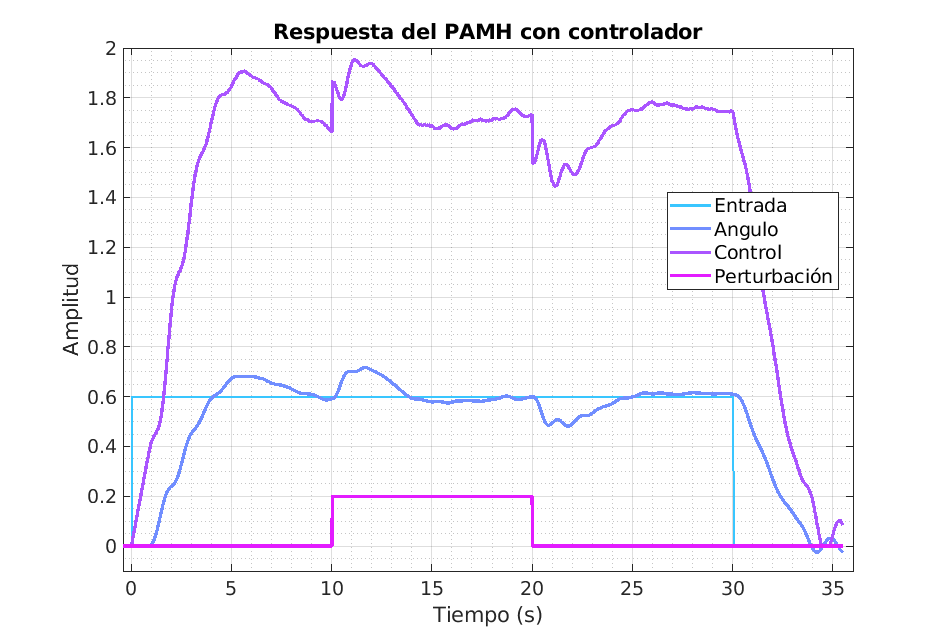
\includegraphics[width=1\linewidth]{fig/PAMH_I_PD.png}
    \caption{Respuesta del sistema PAMH controlado con I-PD}
    \label{fig:pamhsys_ipd}
\end{figure}

\subsection{Control por REI (LQR)}

Por ultimo, con el controlador REI, se obtuvo el comportamiento de la Fig. \ref{fig:pamhsys_ss_lqr}, siendo en cuanto al angulo la más estable de todas, con un tiempo de estabilización de 4.42 s, además de no presentar sobreimpulso completamente.

\begin{figure}[htbp]
    \centering
    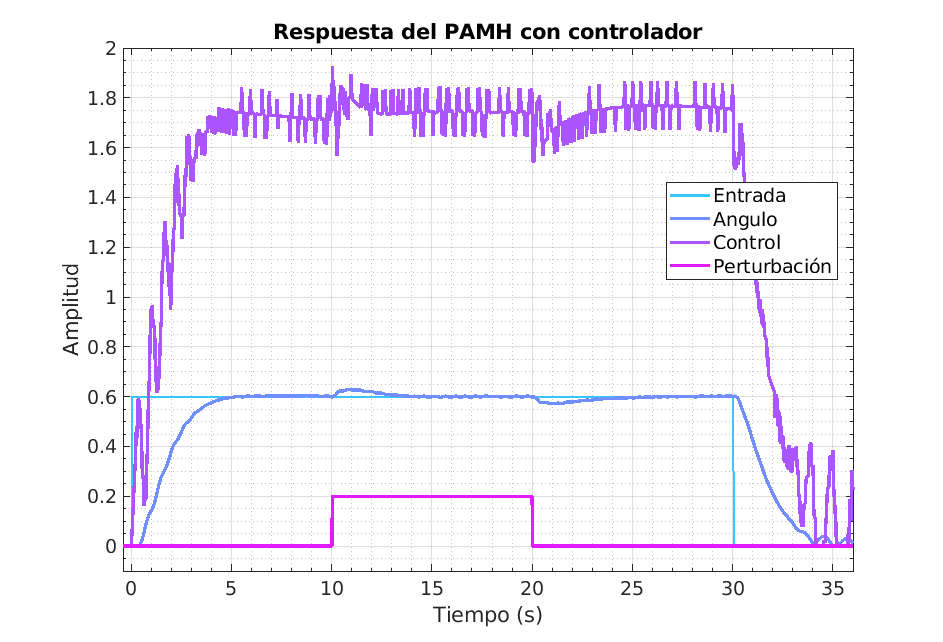
\includegraphics[width=1\linewidth]{fig/PAMH_SS_LQR.png}
    \caption{Respuesta del sistema PAMH controlado con REI-LQR}
    \label{fig:pamhsys_ss_lqr}
\end{figure}

En la Tabla \ref{tab:comp_reg} se denotan los aspectos más importantes respecto a las respuestas obtenidas experimentalmente.

\begin{table}[htbp]
\centering
\caption{Comparacion de Reguladores implementados}
\label{tab:comp_reg}
\begin{tabular}{|l|c|c|c|}
\hline
Caracteristica \textbackslash Regulador & PID              & I-PD & REI         \\ \hline
Tiempo de Estabilización (s)            & 4.46 (presenta oscilaciones) & 8.78 & 4.42        \\ \hline
Porcentaje de Amortiguamiento (\%)      & 8.5              & 14   & No presenta \\ \hline
Elimina Perturbaciones                  & Sí               & Sí   & Sí          \\ \hline
\end{tabular}
\end{table}

\newpage

\section{Análisis de resultados}

En la etapa de simulación, los seis controladores evaluados cumplieron con los requerimientos deseados, lo que indica que, teorícamente, los controladores fueron diseñados de manera correcta con los métodos utilizados.

El PID manual obtuvo un tiempo de estabilización de 4.67 s y un sobreimpulso del 0.45\%, gracias a la ubicación adecuada de ceros para cancelar polos del sistema, lo que concuerda con la teoría, donde la ubicación de ceros permite moldear la respuesta transitoria. 

El método IMC para PID, demostró un comportamiento más suave al eliminar el sobreimpulso completamente, aunque disminuyendo la rapidez del sistema por 0.11 segundos. Lo que permite no solo reflejar el balance de diseño entre la estabilidad y velocidad de respuesta al diseñar un controlador en este tipo de sistemas, sino que permite verificar la eficacia de las aplicaciones digitales para el diseño de controladores, al ser igual de eficaces o incluso mejores a los métodos manuales.

En cuanto a los controladores I-PD y REI, los resultados fueron consistentes con el comportamiento esperado, ya que el LQR permitió obtener ganancias que ponderan adecuadamente los estados, resultando en una respuesta rápida, sin sobreimpulso y con buen rechazo a perturbaciones. Cabe destacar que el controlador REI con el método LQR, mostró un tiempo de estabilización de 4.42 s, sin sobreimpulso, y una gran robustez frente a perturbaciones, siendo el que más se apega al ideal teórico y el que físicamente y gráficamente se observó que mostraba una mejor estabilización.

El I-PD por Ackermann, pese a cumplir los requerimientos en simulación, en su implementación experimental presentó una respuesta más lenta de 8.78 s y con un sobreimpulso de 14\%. Según Ogata \cite{ogata2010}, este tipo de diferencias puede deberse al uso de técnicas de ubicación de polos si no se considera correctamente la sensibilidad del sistema a perturbaciones o el retardo de la planta. Otra posibilidad está en el coeficiente $N$ del controlador para simulación 5 fue suficiente para eliminar las ondulaciones, sin embargo, en la implementación física el coeficiente no parece ser suficiente para eliminar dichas ondulaciones. 

El desempeño del PID por IMC en implementación experimental mostró oscilaciones no previstas en la simulación, lo que indica que aunque el modelo identificado representa adecuadamente el sistema en el entorno simulado, no capta completamente las dinámicas no lineales y perturbaciones físicas presentes en la planta real.

El método con mejor resultado en comparación al resto de controladores fue el REI con LQR, tanto en simulación como en la práctica, además basado en la teoría se sabe que el enfoque LQR no solo considera los estados del sistema, sino que minimiza un índice de desempeño integral, permitiendo lograr un equilibrio entre rapidez, respuesta transitoria y su estabilidad, además el uso de realimentación de estados con un integrador elimina el error de estado estacionario y mitiga perturbaciones de forma efectiva.

\section{Conclusiones}
\begin{itemize}
\item Todos los controladores diseñados cumplieron teóricamente con los requerimientos, además de demostrar su funcionamiento en simulación con la herramienta de Simulink, lo que valida la correcta aplicación y sencillez de diseño de los métodos PID, I-PD y REI en simulación.

\item El PID por IMC demostró que los métodos automáticos computarizados son eficaces y generan resultados comparables o superiores a los diseños manuales, con respuestas más estables y sin sobreimpulso.

\item El método LQR para el diseño de I-PD y REI produjo resultados consistentes, destacando especialmente el REI-LQR, que logró el mejor desempeño general, tanto en simulación como en implementación.

\item El I-PD por Ackerman presentó deficiencias en la implementación, como lentitud en la estabilización, posiblemente debido a una sensibilidad excesiva a perturbaciones y una selección de polos poco robusta frente al retardo de la planta, así como la posible falta de variación y prueba del coeficiente N.

\item Las diferencias entre simulación e implementación, especialmente en el caso del PID IMC e I-PD Acker, reflejan las limitaciones de los modelos lineales frente al comportamiento no lineal real del sistema PAMH.

\item El REI con LQR fue el controlador más robusto, con la mejor respuesta transitoria y capacidad de rechazo a perturbaciones, validando su superioridad tanto práctica como teórica.
    
\end{itemize}

\section{Referencias Bibliográficas}
\printbibliography[heading=none]

\end{document}